\documentclass{../tufte-handout}

\title{Intro to Linear Dynamical Systems -- Lecture 1}

\author{Pralhad Deshpande  (pralhdes@in.ibm.com)}

%\date{28 March 2010} % without \date command, current date is supplied

%\geometry{showframe} % display margins for debugging page layout

\usepackage{graphicx} % allow embedded images
  \setkeys{Gin}{width=\linewidth,totalheight=\textheight,keepaspectratio}
  \graphicspath{{graphics/}} % set of paths to search for images
\usepackage{amsmath}  % extended mathematics
\usepackage{booktabs} % book-quality tables
\usepackage{units}    % non-stacked fractions and better unit spacing
\usepackage{multicol} % multiple column layout facilities
\usepackage{lipsum}   % filler text
\usepackage{fancyvrb} % extended verbatim environments
  \fvset{fontsize=\normalsize}% default font size for fancy-verbatim environments

% Standardize command font styles and environments
\newcommand{\doccmd}[1]{\texttt{\textbackslash#1}}% command name -- adds backslash automatically
\newcommand{\docopt}[1]{\ensuremath{\langle}\textrm{\textit{#1}}\ensuremath{\rangle}}% optional command argument
\newcommand{\docarg}[1]{\textrm{\textit{#1}}}% (required) command argument
\newcommand{\docenv}[1]{\textsf{#1}}% environment name
\newcommand{\docpkg}[1]{\texttt{#1}}% package name
\newcommand{\doccls}[1]{\texttt{#1}}% document class name
\newcommand{\docclsopt}[1]{\texttt{#1}}% document class option name
\newenvironment{docspec}{\begin{quote}\noindent}{\end{quote}}% command specification environment

\begin{document}

\maketitle% this prints the handout title, author, and date


%\printclassoptions

This document covers lecture 1 from \cite{boyd-lds-2008}.

\section{What is a linear dynamical system?}


\subsection{Continuous-time linear dynamical system}

A continuous time linear dynamical system (CT LDS) is a first order vector differential equation. There are other names for it, e.g., state equations, or `m-input, n-state, p-output' LDS. It looks like this: 

\vspace{0.15in}
$dx/dt = A(t)x(t) + B(t)u(t)$ \footnote{This is sometimes called the dynamics equation.},
\newline
$y(t) = C(t)x(t) + D(t)u(t)$ \footnote{This is sometimes called the measurement or readout equation.} \hspace{0.25in}
\vspace{0.15in}

where: \newline
$t \in \mathbb{R}$ denotes time.  \newline
$x(t)$ is a vector function and is called the state. \footnote{Colloquially, the actual entries of $x_i(t)$ of $x(t)$ are called the states. This is informal slang.} \newline
$u(t)$ is called the input or control. \newline
$y(t)$ is the output. \newline
$A(t) \in \mathbb{R}^{n \times n}$ is the dynamics matrix.\newline
$B(t) \in \mathbb{R}^{n \times m}$ is the input matrix.\newline
$C(t) \in \mathbb{R}^{p \times n}$ is the output or sensor matrix.\newline
$D(t) \in \mathbb{R}^{p \times m}$ is the feedthrough matrix.\newline

We will go through all of this in horrendous detail later in the course. A concise short form of the CT LDS equations is: \newline
\vspace{0.15in}
$\dot x = Ax + Bu, \hspace{0.25in} y = Cx + Du$
\vspace{0.15in}

\textbf{Time-invariant LDS:} Most LDS are time-invariant, i.e., $A$, $B$, $C$, $D$ are constant and do not depend on $t$.

 \textbf{Autonomous LDS:}  Sometimes there is no input or control, i.e., no $u$. This implies that there is no $B$ or $D$. These are called autonomous LDS. Essentially, this system goes by itself without needing any input. 
 
 \textbf{No Feedthrough LDS:} Very often there is no feedthrough, i.e., $D=0$. So you get what is very simple. 
 
 \textbf{SISO and MIMO systems:} if $u(t)$ and $y(t)$ are scalar, the system is called SISO. When input and output dimensions are more than one, the system is called MIMO. This is a little bit silly. It is a holdover from the time when it was a big deal to have multiple inputs and outputs. At this time, wireless communications is probably going through the very end of the MIMO stage of development. This was very hot 10 years ago. Other fields have done this decades and decades ago. Some fields have not yet reached the MIMO stage but they soon will. 


\subsection{Discrete-time linear dynamical system}



Discrete-time linear dynamical system (DT LDS) is a recursion. Instead of a derivative, it is simply an update equation. It has the form: 

\vspace{0.15in}
$x(t+1) = A(t)x(t) + B(t)u(t)$ \footnote{The next state is obtained by multiplying the current state by the matrix $A(t)$ and to that you add something that is related to an input.} \newline
$y(t) = C(t)x(t) + D(t)u(t)$
\vspace{0.15in}

where: \newline
$t \in \mathbb{Z} = \{0, \pm 1, \pm 2, ...\}$ \footnote{Here time is an integer. It could be a sample or a period for example in the stock market.}\newline
In this case signals $x$, $u$, $y$ are sequences. In the CT case they were functions. So this is nothing but a first order vector recursion. 

\section{Why study linear systems?}

Applications of linear systems come up everywhere. The first application was in automatic control systems (aerospace). It hit signal processing 15 - 20 years ago. It hit communications big time about 10 years ago. Most models in economics and finance are based on LDS. LDS plays a very important role in circuit analysis, simulation and design. It comes up in mechanical and civil engineering. You see it a lot in dynamics of structures and all sorts of other stuff. It comes up in navigation and guidance, e.g., GPS. Comes up in machine learning as well. 

Also, if you combine what you learn in this course with what you learn in Probability and Statistics you will be able to apply that to tonnes and tonnes of fields. The usefulness of this material scales with available computing power, i.e., it scales exponentially with Moore's law. This material was ultra-hi-end 30 years ago and only a handful of math Ph.D. students would study this material. But today this is undergraduate material. 

\section{Nonlinear Dynamical Systems}

Many dynamical systems are nonlinear. But it is still important to study linear systems. Most techniques for nonlinear systems are based on linear methods. Methods for linear systems often work unreasonably well, in practice, for nonlinear systems. If you do not understand linear dynamical systems, you certainly can't understand nonlinear dynamical systems. 

\section{Example: Input Design}
Let us consider a few examples. We will only work with ideas and not get down to the details for now. Let's consider a specific system: \newline

\vspace{0.15in}
$\dot x = Ax, \hspace{0.25in} y = Cx$\newline
with $x(t) \in \mathbb{R}^{16}, \hspace{0.25in} y(t) \in \mathbb{R}$ 
\vspace{0.15in}

This is a 16 state single-output system. The output is a scalar. This happens to be a model of a lightly damped mechanical system. It has 8 generalized positions and the dynamics is what happens when you poke it or when an earthquake excites it and then the whole structure wiggles around. The output would be the specific displacement in some axis at some point in the structure. 


\begin{marginfigure}
  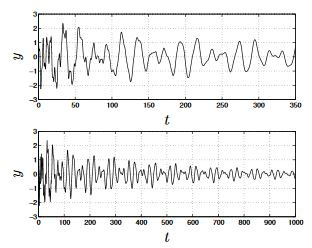
\includegraphics[width=\linewidth]{output_lightly_damped_structure}
  \caption{Typical output when the structure is excited.}
  \label{fig:output_lightly_damped_structure}
\end{marginfigure}

If you were given the first 100 samples of the output and were not told what it was, it is unlikely you would be able to guess what this signal would be doing at t = 1000. This output, and indeed the output of any linear dynamical system can be spectrally decomposed into complex frequencies. The output waveform that you see in Figure~\ref{fig:output_lightly_damped_structure} can be decomposed into modal components shown in Figure~\ref{fig:modal_components_output_lightly_damped_structure}.

\begin{marginfigure}
  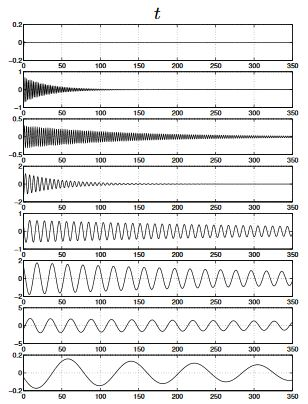
\includegraphics[width=\linewidth]{modal_components_output_lightly_damped_structure}
  \caption{Modal components of output. If you add these components you will get the output waveform shown in Figure~\ref{fig:output_lightly_damped_structure}}
  \label{fig:modal_components_output_lightly_damped_structure}
\end{marginfigure}

If instead of first 100 samples of the waveform in Figure~\ref{fig:output_lightly_damped_structure}, you were given the first 100 samples of the decomposed signal, you would have no problem in predicting what the signal would look like at t = 1000. 

Now lets look at input design. We are going to add two inputs and two outputs to the system. You can imagine a building and put two hydrolic actuators on it. And now we measure the displacement at two other places. So now we have a 2-input, 2-output system: \newline

\vspace{0.15in}
$\dot x = Ax + Bu, \hspace{0.25in} y = Cx, \hspace{0.25in} x(0) = 0$\newline
where: $B \in \mathbb{R}^{16 \times 2},  C \in \mathbb{R}^{2 \times 16}$  (Same $A$ as before.)
\vspace{0.15in}

\textbf{Problem:} \footnote{This is a control or input problem. Choose an input that makes what you want to happen, happen.} find the appropriate input $u \in \mathbb{R}^{2}$ that brings the output to some desired point $y_{des} = (1, -2)$ 

This is a very common problem. For example, in a disc drive the head gets a command to move from track 22 to track 232 and it has to do that in a short amount of time.

\textbf{Simple approach:} consider the static conditions. In this case $u, x, y$ are constant. \newline 

$\dot x = 0 = Ax + Bu_{static}, \hspace{0.25in} y = y_{des} = Cx$

\vspace{0.25in}

We can solve for $u$ to get: 

$u_{static} = (-CA^{-1}B)^{-1}y_{des} = \begin{bmatrix} -0.63\\ 0.36 \end{bmatrix}$

\begin{marginfigure}
  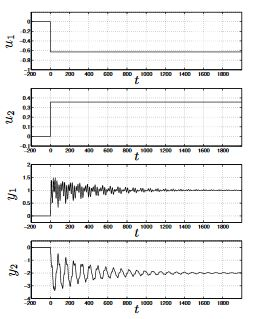
\includegraphics[width=\linewidth]{simple_approach}
  \caption{At about t = 1500 the outputs converge to 1 and -2.}
  \label{fig:simple_approach}
\end{marginfigure}

\newpage
\textbf{Fast convergence: } As seen in Figure~\ref{fig:fast_convergence} fast convergence is possible using clever input waveforms. Note that the two inputs are far from intuitive. No one can guess them. And \textit{this} is what this class is about! Also note that we are restricting the range of input between -0.63 and 0.36.

\begin{marginfigure}
  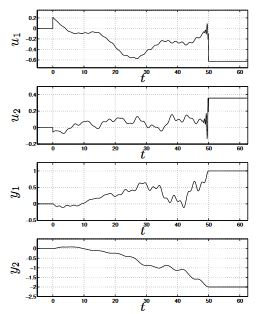
\includegraphics[width=\linewidth]{fast_convergence}
  \caption{Convergence at t = 50 using clever input design. }
  \label{fig:fast_convergence}
\end{marginfigure}


\textbf{Faster convergence: } As seen in Figure~\ref{fig:faster_convergence} faster convergence is possible. We can use larger inputs to do this. 

\begin{marginfigure}
  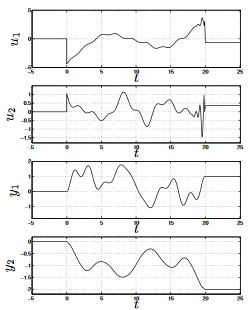
\includegraphics[width=\linewidth]{faster_convergence}
  \caption{Convergence at t = 20 using larger inputs.}
  \label{fig:faster_convergence}
\end{marginfigure}

\newpage
\section{Example: Estimation / Filtering}

\begin{marginfigure}
  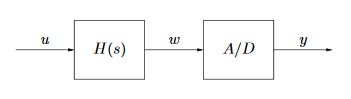
\includegraphics[width=\linewidth]{estimation}
  \caption{.}
  \label{fig:estimation}
\end{marginfigure}

\begin{marginfigure}
  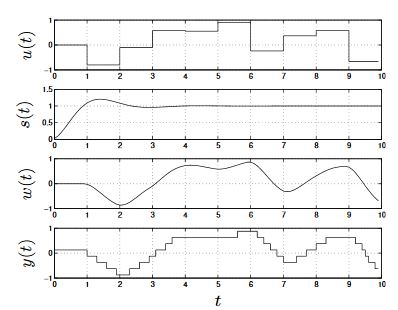
\includegraphics[width=\linewidth]{estimation_typical_behavior}
  \caption{.}
  \label{fig:estimation_typical_behavior}
\end{marginfigure}

\begin{marginfigure}
  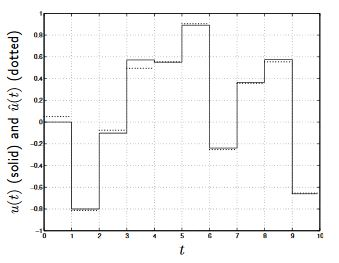
\includegraphics[width=\linewidth]{estimation_better_approach}
  \caption{.}
  \label{fig:estimation_better_approach}
\end{marginfigure}



57:35


\bibliography{../lecture-notes}
\bibliographystyle{plainnat}



\end{document}
